\documentclass{beamer}
\usepackage[T1]{fontenc}
%% \usepackage{DejaVuSansCondensed}
%% \usepackage[defaultsans]{opensans}
\usepackage[scaled=0.8]{DejaVuSansMono}
%% \usepackage{amsfonts}
%% \usepackage{arev}
%% \mode<presentation>
\usepackage{quattrocento}

%% Theming
\usetheme{Goettingen}
%% \usecolortheme{dove}
\usefonttheme{structurebold}
\setbeamertemplate{navigation symbols}{}

%% Extra stuff
\usepackage{graphics}

%% Front matter
\title[Packrat Parsing]{Packrat Parsing:
  \\a Practical Linear-Time
  Algorithm with Backtracking}
\subtitle{Bryan Ford \\
  MIT Master's Thesis 2002}
\author[Sean Cribbs]{\Large Sean Cribbs \\
  \small{@seancribbs}}
\date[Papers We Love Chicago]{Papers We Love Chicago \#1 \\
  20 August 2014}

\begin{document}

\begin{frame}
  \maketitle
\end{frame}

\begin{frame}
\frametitle{About Me}
\begin{itemize}
\item Engineer at Basho, Conference Junkie
\item Favorite CS class was \textit{Compiler Construction}
\item Creator of \texttt{neotoma}, packrat-parser toolkit for Erlang
\end{itemize}
\end{frame}

\begin{frame}
\frametitle{Outline}
\tableofcontents
\end{frame}

%% Background section
\section[Background]{Languages, Grammars, Parsing}
\begin{frame}{What is parsing?}
  \begin{itemize}
  \item Languages express information linearly, as sequences of
    symbols
  \item Applications that use languages must derive higher-level
    constructs
    \begin{itemize}
    \item words, phrases, clauses, sentences, expressions, statements,
      ...
    \end{itemize}
  \item This is called \alert{syntax analysis} or \alert{parsing}
  \end{itemize}
\end{frame}

\begin{frame}{Terminology}
  \begin{itemize}
  \item Language
  \item Grammar
  \item Terminal/Nonterminal
  \item Rule (production, reduction)
  \item Top-down parsing (recursive descent)
  \item Bottom-up parsing (shift/reduce)
  \end{itemize}
\end{frame}

\begin{frame}{Who is this?}
\centering
  \begin{figure}
    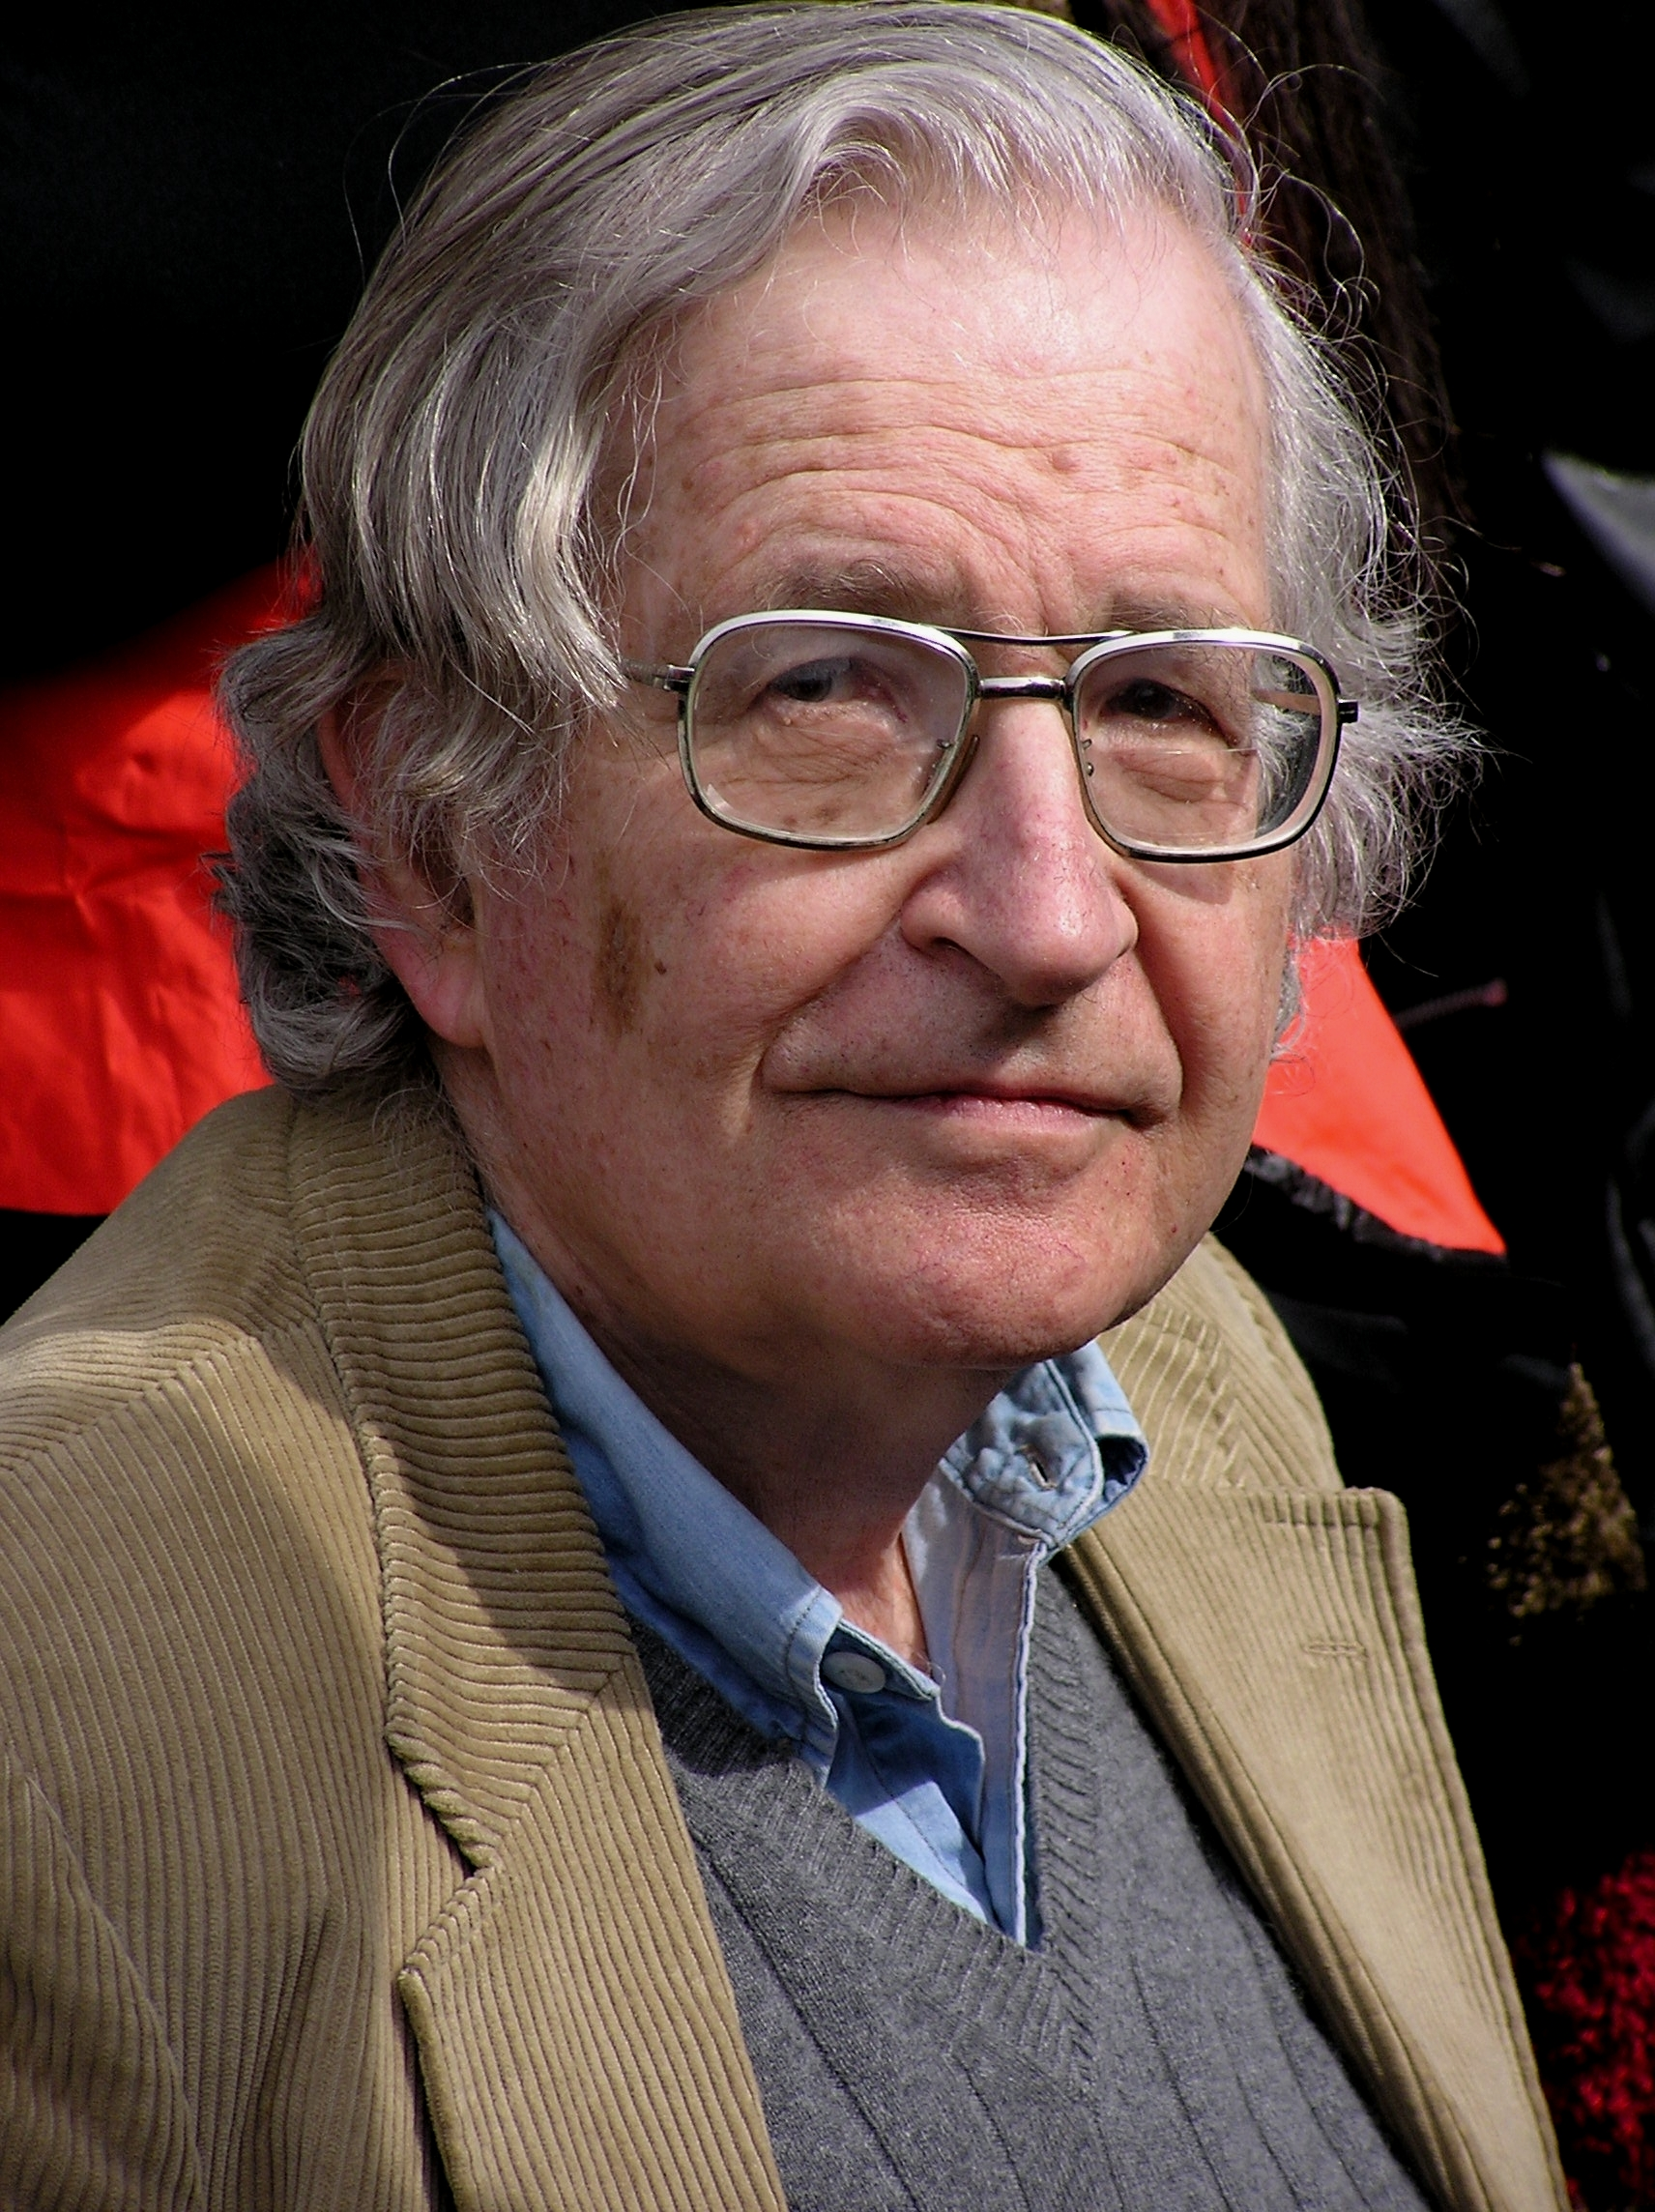
\includegraphics[height=70mm]{Chomsky.jpg}
    \caption{\small \copyright~Duncan Rawlinson, CC BY 2.0}
  \end{figure}
\end{frame}

\begin{frame}{Chomsky's Hierarchy}
  \begin{figure}
    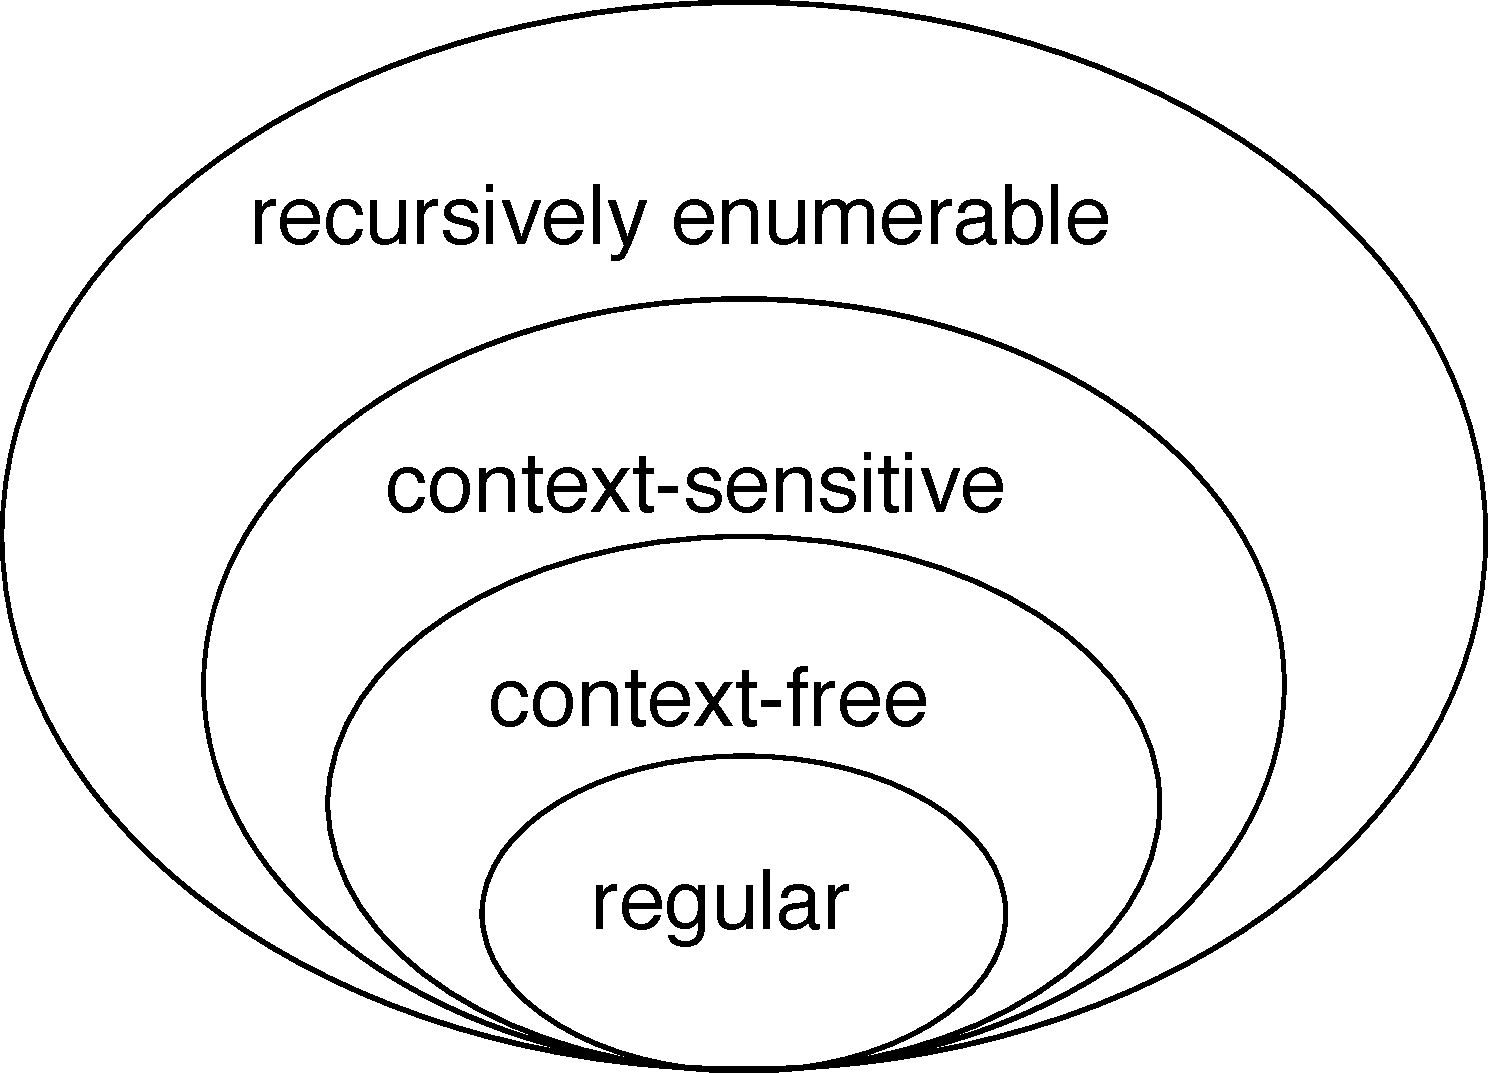
\includegraphics[width=80mm]{Chomsky-hierarchy.pdf}
    \caption{\copyright~J. Finkelstein, CC BY-SA 3.0}
  \end{figure}
\end{frame}

\begin{frame}{Regular}
  \begin{itemize}
    \item Very popular in practical use via \textit{regular expressions}
    \item Recognizable via finite-state automata
    \item Used in scanning, aka ``lexical analysis''
  \end{itemize}
  \begin{figure}
    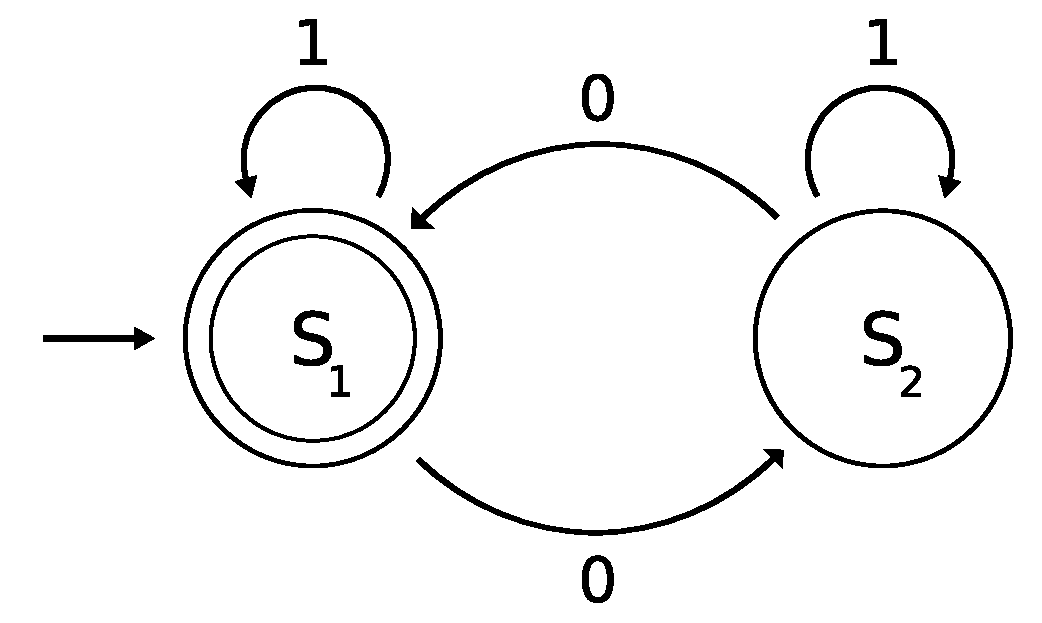
\includegraphics[height=30mm]{DFAexample.pdf}
    \caption{Deterministic finite-state automaton (DFA)}
  \end{figure}
\end{frame}

\begin{frame}{Context-free}
  \begin{itemize}
    \item What we usually think of when discuss ``grammars'' - tools
      like yacc/Bison/ANTLR
    \item Unlike Regular languages, \textit{can} express recursive
      constructs
    \item Recognizable via pushdown-automata (stack-based)
    \item Used in parsing, aka ``syntax analysis''
  \end{itemize}
  \begin{gather}
    S \rightarrow aSb ~|~ \epsilon \\
    \epsilon~|~ab~|~aabb~|~aaabbb~|~... \\
    S \rightarrow a^* b^* \\
    a~|~b~|~ab~|~aab~|~aabb~|~aabbb~|~...
  \end{gather}
\end{frame}

\begin{frame}{Problems with CFGs}{for machine-readable languages}
  \begin{itemize}
    \item Focused on \textit{generating} strings, not \textit{recognizing}
    \item Often ambiguous: both \textit{locally} and \textit{globally},
      frequently augmented with manual disambiguation
    \item Generally require separate scanning step
    \item Predictive and shift/reduce parsing algorithms only work
      with restricted CFGs
  \end{itemize}
\end{frame}

\section[Contributions]{This Thesis' Contributions}
\begin{frame}{This Thesis' Contributions}
  \begin{enumerate}
    \item Makes \textbf{Top-Down Parsing Language} a practical notation
    \item \textbf{Packrat-parsing} algorithm
    \item A TDPL/Packrat-parser generator for Haskell, \textbf{Pappy}
  \end{enumerate}
\end{frame}

\begin{frame}{TDPL}{Top-Down Parsing Language}
  \begin{itemize}
    \item Formalism for describing top-down parsing algorithms (aka
      recursive-descent)
    \item Expresses how to \textit{read} strings rather than \textit{write}
      them
    \item Also known as \textit{parsing expression grammar} (PEG)
    \item Fundamentally \textbf{unambiguous} via \textit{ordered choice}
  \end{itemize}
\end{frame}

\begin{frame}{PEG/TDPL constructs}
  \begin{tabular*}{.75\textwidth}[t]{|l|c|}
    Empty string               & $()$ \\[5pt]
    Terminal                   & $a$ \\[5pt]
    Nonterminal                & $A$ \\[5pt]
    Sequence                   & $e_1~e_2~e_3~...$ \\[5pt]
    Ordered-choice             & $e_1 \slash e_2 \slash e_3 \slash ...$ \\[5pt]
    Greedy repetition          & $e^*$ \\[5pt]
    Greedy positive repetition & $e+$ \\[5pt]
    Optional                   & $e?$ \\[5pt]
    Followed-By                & $\&(e)$ \\[5pt]
    Not-Followed-By            & $!(e)$
  \end{tabular*}
\end{frame}

\begin{frame}{PEG advantages}
  \begin{itemize}
  \item Tokenization can be done inline (scannerless parsing)
  \item Constructs like ``reserved words'' can be expressed directly
  \item Associativity is more directly controlled
  \end{itemize}
\end{frame}

\begin{frame}[fragile]{Longest-match disambiguation}{The dangling else
    problem}
\begin{verbatim}
  IF a THEN  IF b THEN c  ELSE d
\end{verbatim}
\pause
\begin{verbatim}
  IF a THEN (IF b THEN c) ELSE d

  IF a THEN (IF b THEN c  ELSE d)
\end{verbatim}
\pause
\begin{itemize}
  \item Languages usually pick the latter.
  \item Ordered-choice makes this disambiguation explicit:
\end{itemize}
\begin{verbatim}
  if_stmt <- "IF" e "THEN" s "ELSE" s / 
             "IF" e "THEN" s
\end{verbatim}
\end{frame}

\begin{frame}{PEG limitations}
  \begin{itemize}
    \item Cannot express ambiguous syntax
    \item Some CFGs have no corresponding PEG
    \item Repetition is always greedy, workaround with predicates
    \item Left-recursion is erroneous*
  \end{itemize}
\end{frame}

\begin{frame}[fragile]{Parsing}
Consider the PEG:
\begin{verbatim}
  Additive  <- Multitive `+' Additive / 
               Multitive
  Multitive <- Primary `*' Multitive / 
               Primary
  Primary   <- `(' Additive `)' / Decimal
  Decimal   <- `0' / ... / `9' 
\end{verbatim}
\end{frame}

\begin{frame}[fragile]{Simple Top-Down Parser}{Recursive Descent with Backtracking}
\begin{verbatim}
data Result v = Parsed v String | NoParse
\end{verbatim}
\pause
\begin{verbatim}
-- calls itself and pMultitive
pAdditive  :: String -> Result Int 

-- calls itself and pPrimary
pMultitive :: String -> Result Int 

-- calls pAdditive and pDecimal
pPrimary   :: String -> Result Int 

-- consumes a digit
pDecimal   :: String -> Result Int
\end{verbatim}
\end{frame}

\begin{frame}[fragile]{Simple Top-Down Parser}{Recursive Descent with
    Backtracking}
\begin{verbatim}
-- Parse an additive-precedence expression 
pAdditive :: String -> Result Int 
pAdditive s = alt1 where
  -- Additive <- Multitive `+' Additive 
  alt1 = case pMultitive s of
           Parsed vleft s' -> 
             case s' of
               (`+':s'') ->
                 case pAdditive s'' of
                   Parsed vright s''' ->
                     Parsed (vleft + vright) s'''
                   _ -> alt2
               _ -> alt2
           _ -> alt2
\end{verbatim}
\end{frame}

\begin{frame}[fragile]{Simple Top-Down Parser}{Recursive Descent with
    Backtracking}
\begin{verbatim}
-- continued from previous slide

  -- Additive <- Multitive 
  alt2 = case pMultitive s of
           Parsed v s' -> Parsed v s'
           NoParse -> NoParse
\end{verbatim}
\pause
\begin{itemize}
\item On a plain \texttt{Multitive} expression, \alert{\textbf{we compute that twice!}}
\item Worst-case backtracking can result in exponential parse times:
  $O(2^n)$
\end{itemize}
\end{frame}

\begin{frame}[fragile]{Tabular Parsing}{Figure 3-2}
\small
\begin{tabular*}{80mm}{l*{8}{c}}
  column    & C1 & C2 & C3 & C4     & C5 & C6     & C7 & C8 \\[5pt]
  \cline{2-9}\\[-8pt]
  pAdditive &    &    &    & (7,C7) & X  & (4,C7) & X  & X 
  \\[5pt]
  pMultitive &    &    & $\uparrow$   & (3,C5) & X  & (4,C7) & X  & X  \\[5pt]
   pPrimary &    & $\leftarrow$    & \textcircled{\tiny ?}   & (3,C5) & X  & (4,C7) & X  & X  \\[5pt]
   pDecimal &    &   & X  & (3,C5) & X  & (4,C7) & X  & X  \\[5pt]
  \cline{2-9}\\[-8pt]
   input & 2  & *  & (  & 3      & +  & 4      & )  & (end)
\end{tabular*}
\pause
\bigskip
\begin{itemize}
\item Linear parse time (proportional to input)
\item All results are precomputed and can be referred to directly
  rather than recursing
\pause
\item \textbf{BUT} It computes \textbf{way more} results than
  necessary!
\item \textbf{AND} The order in which rules are computed must be
  carefully chosen!
\end{itemize}
\end{frame}

\begin{frame}{Packrat Parsing}
  \begin{itemize}
  \item \textbf{Lazy} version of the tabular algorithm, computing
    results only as needed
  \item Computes results in the same order as a recursive-descent
    parser
  \item \textbf{BUT} it doesn't compute the same ``cell'' more than
    once, unlike the naive backtracking parser
    \pause
  \item \alert{All of this is accomplished with plain algebraic data types in
    Haskell!}
  \end{itemize}
\end{frame}

\begin{frame}[fragile]{Making a Packrat Parser}{Modifying our existing one}
\begin{verbatim}
-- A column in our table
data Derivs = Derivs { dvAdditive  :: Result Int 
                       dvMultitive :: Result Int 
                       dvPrimary   :: Result Int 
                       dvDecimal   :: Result Int 
                       dvChar      :: Result Char }
\end{verbatim}
\pause
\begin{verbatim}
-- Modify the Result type
data Result v = Parsed v Derivs 
                | NoParse
\end{verbatim}
\pause
\begin{verbatim}
-- And the parsing functions
pAdditive  :: Derivs -> Result Int 
pMultitive :: Derivs -> Result Int 
pPrimary   :: Derivs -> Result Int 
pDecimal   :: Derivs -> Result Int 
\end{verbatim}
\end{frame}

\begin{frame}[fragile]{Rewriting \texttt{pAdditive}}
\begin{verbatim}
pAdditive :: Derivs -> Result Int
pAdditive d = alt1 where
  -- Additive <- Multitive `+' Additive 
  alt1 = case dvMultitive d of
           Parsed vleft d' -> 
             case dvChar d' of
               Parsed `+' d'' ->
                 case dvAdditive d'' of
                   Parsed vright d''' ->
                     Parsed (vleft + vright) d'''
                   _ -> alt2
               _ -> alt2
           _ -> alt2

  -- Additive <- Multitive
  alt2 = dvMultitive d
\end{verbatim}
\end{frame}

\begin{frame}[fragile]{Tie-Up the Structure}{with data-recursion}
\begin{verbatim}
-- Create a result matrix for an input string
parse :: String -> Derivs
parse s = d where
    d    = Derivs add mult prim dec chr 
    add  = pAdditive d
    mult = pMultitive d
    prim = pPrimary d
    dec  = pDecimal d 
    chr =  case s of
             (c:s') -> Parsed c (parse s') 
             [] -> NoParse
\end{verbatim}
\end{frame}

\begin{frame}{Derivs expanded}
\begin{figure}
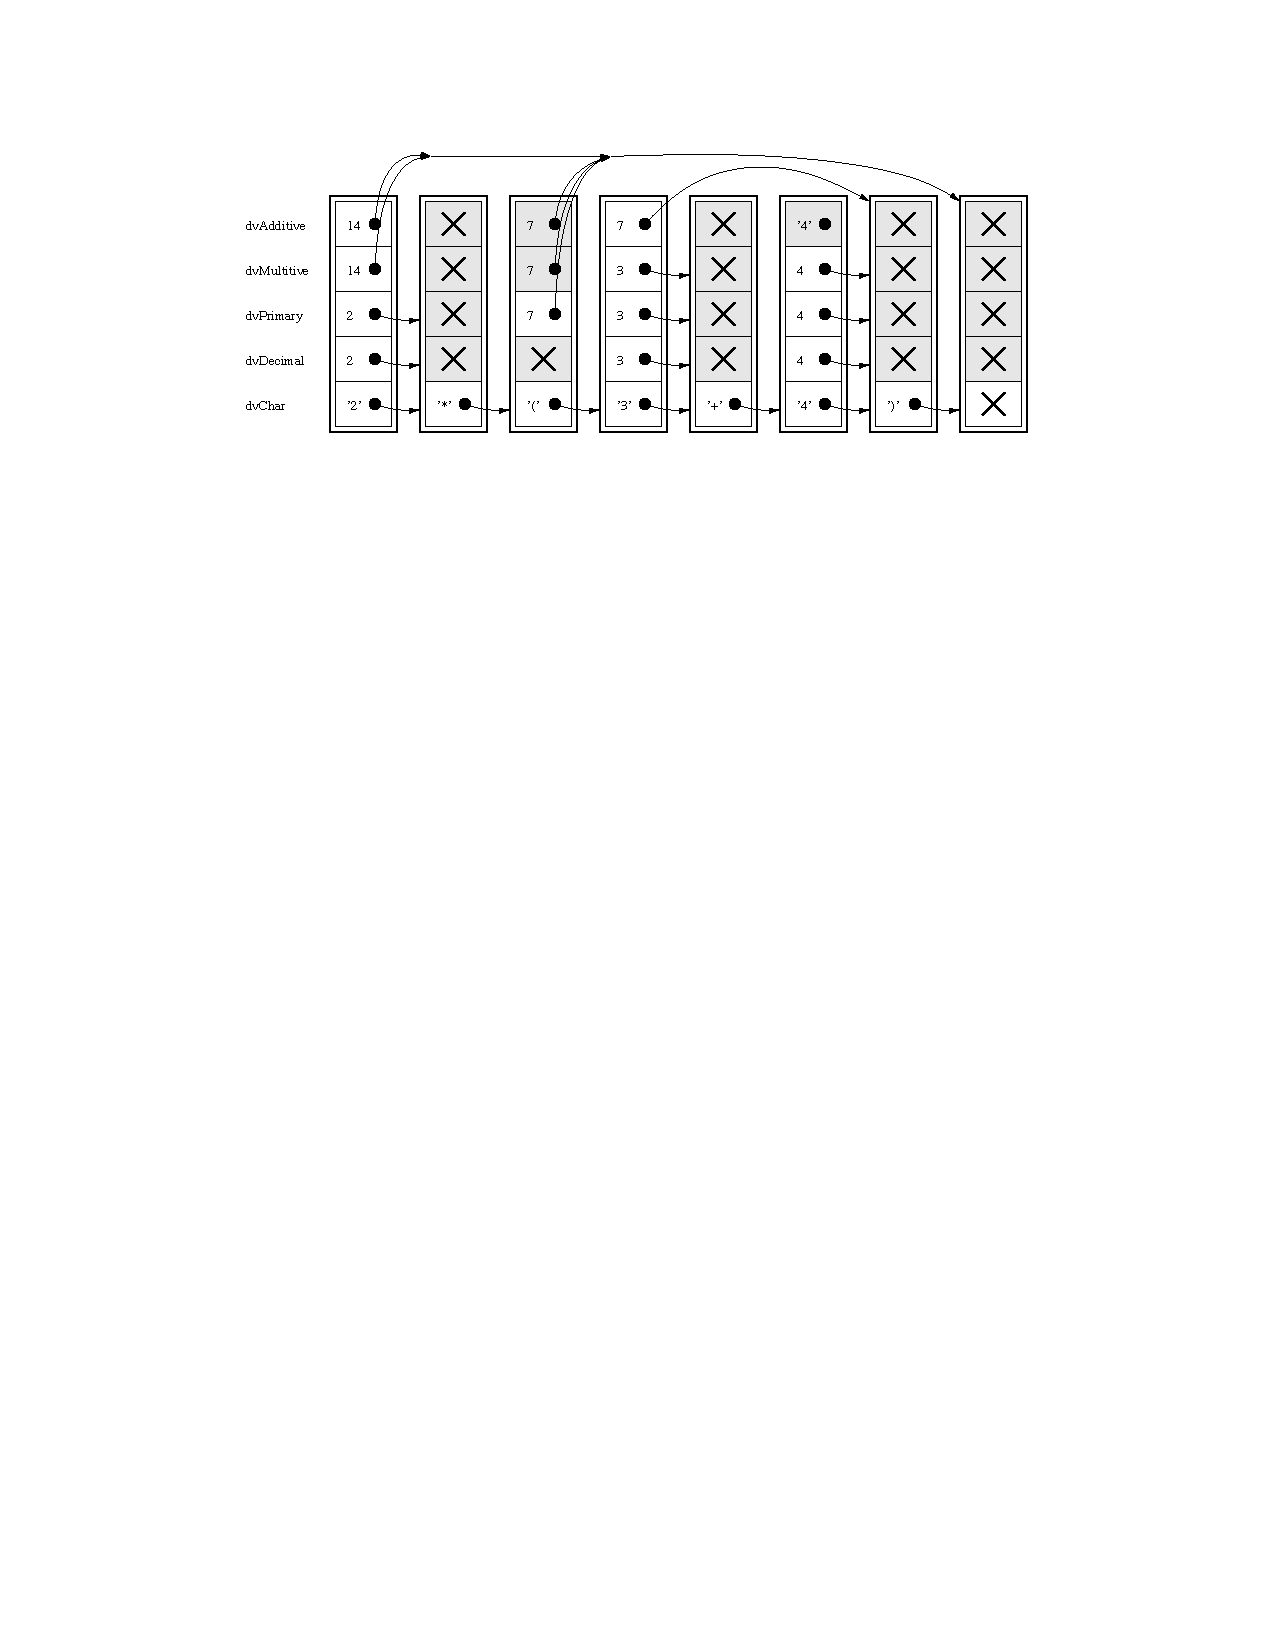
\includegraphics[width=\textwidth]{memotable.pdf}
\caption{Parsing \texttt{``2 * (3 + 4)''}}
\end{figure}
\end{frame}

\begin{frame}{mindblown.hs}
\center

\includegraphics[width=.8\textwidth]{mindblown.jpeg}
\end{frame}

\begin{frame}{Limitations of Packrat Parsing}
  \begin{itemize}
  \item Language must be unambiguous
  \item Limited state
  \item Space consumption is large
  \end{itemize}
\end{frame}

\begin{frame}{Stuff I'm not covering}{but is still awesome}
  \begin{itemize}
  \item Monadic Packrat Parsing
  \item Error Handling
  \item Maintaining Input Position Information
  \item Stateful Parsers
  \item \textit{Pappy}, the parser generator
  \end{itemize}
\end{frame}

\section{Why I Love It}
\begin{frame}{Why I Love It}
  \begin{itemize}
  \item Simple principles, powerful results
  \item Written in a very thorough, approachable style
  \item Very honest about tradeoffs
    \pause
  \item I hardly use regular expressions for anything complicated
    anymore.
  \item \texttt{neotoma} is almost more popular than \texttt{yecc} in
    Erlang open-source projects
  \end{itemize}
\end{frame}

\section{Discussion}
\begin{frame}{Further Reading}
  \begin{thebibliography}{a}
    \beamertemplateonlinebibitems
    \bibitem[Ford, 2014]{a}
      B.~Ford
      \newblock The Packrat Parsing and Parsing Expression Grammars
      Page
      \newblock \texttt{http://bford.info/packrat/}
  \end{thebibliography}
\end{frame}


\begin{frame}{Discussion}
  \begin{itemize}
  \item Questions?
  \item Comments?
  \item Ideas?
  \end{itemize}
\end{frame}

\end{document}
